\documentclass{standalone}
\usepackage{pgfplots}
\pgfplotsset{compat=1.18}

\begin{document}

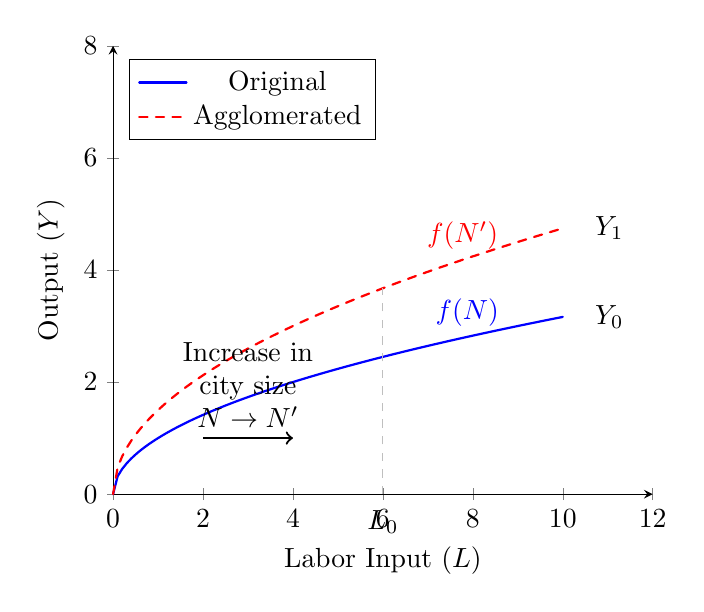
\begin{tikzpicture}
\begin{axis}[
    axis lines = left,
    xlabel = {Labor Input ($L$)},
    ylabel = {Output ($Y$)},
    xmin=0, xmax=12,
    ymin=0, ymax=8,
    grid=none,
    legend pos=north west,
    clip=false
]

% Original production function (N)
\addplot[
    domain=0:10,
    samples=100,
    color=blue,
    thick,
    line cap=round
] {sqrt(x)} node[pos=0.8, above] {$f(N)$};

% Shifted production function (N')
\addplot[
    domain=0:10,
    samples=100,
    color=red,
    thick,
    dashed,
    line cap=round
] {1.5*sqrt(x)} node[pos=0.8, above] {$f(N')$};

% Vertical reference line
\addplot[dashed, gray!50] coordinates {(6,0) (6, {1.5*sqrt(6)})};

% Labels and annotations
\node at (axis cs:6, -0.5) {$L_0$};
\node at (axis cs:10.5, {sqrt(10)}) [right] {$Y_0$};
\node at (axis cs:10.5, {1.5*sqrt(10)}) [right] {$Y_1$};

\draw[->, thick] (axis cs:2, 1) -- (axis cs:4, 1) 
    node[midway, above, align=center] {Increase in\\city size\\$N \rightarrow N'$};

\legend{Original, Agglomerated}
\end{axis}
\end{tikzpicture}

\end{document}